\newpage

\section{Návrh riešenia}

Implementácia je postavená okolo dvoch základných funkcionalít, ktoré sa budú navzájom dopĺňať, pôjde vyhľadávanie v hudobných dokumentoch ktorého hlavnou úlohou bude naplniť používateľské profily preferenciami a zostavovanie spevníkov na základe týchto preferencií. 

\subsection{Vyhľadávanie hudobných dokumentov}

Vyhľadávanie bude pracovať nad už existujúcou databázou hudobných dokumentov. V podstate bude využívať už funkčné vyhľadávanie na tejto stránke, akurát na základe používateľových preferencií rozšíri jeho vyhľadávacie reťazce o ďalšie slová ktoré presnejšie špecifikujú používateľov zámer.

\begin{figure}\begin{center}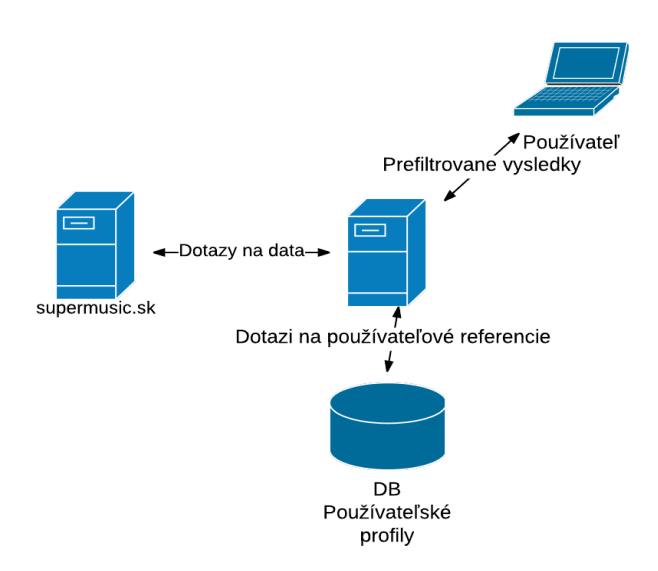
\includegraphics[scale=0.55]{servers}
\caption{Náčrt funkčnosti aplikácie.}\label{Náčrt funkčnosti aplikácie}
\end{center}\end{figure}

\subsection{Zostavenie spevníka}

Aplikácia bude podporovať funkcionalitu automatického generovania spevníka, kedy si používateľ zvoli používateľov s ktorými si chce ísť zahrať a aplikácia automatický vygeneruje spevník zložený s nejpreferovanejších hudobných diel daných používateľov.

\subsection{Krawler ?}

Tento komponenet prehľadáva databázu ktorá je cieľom môjho odporúčača,
využíva k tomu abecedne zobrazenie záznamov databázy.
Databáza sa nedá zobraziť od do,
takže granularitu zobrazenie stránok som musel určiť pokusom,
najskôr som si zobrazoval všetky troj písmenkove názvy,
čo bolo 30*26*26 zobrazení (20280), čo ale trvalo príliš dlho,
tak som v tretej sade prehľadával iba každé štvrté písmenko, čo zredukovalo počet stranok na 3380.

\subsection{Indexing}

Jestvuje veľa spôsobov ako sa dá označovať a vyhľadať obsah, ja som sa počas prieskumu zameral na try:

\paragraph{Priama tagovacia tabuľka}

Vytvoril som tabuľku tagov, kde bol každý tag fyzický priamo vložený spolu z id dokumentu ku ktoremu sa viaže,
tento prístup ale nebol dostatočne rýchli na vygenerovanie, ani na vyhľadávanie. Pri vyhľadávaní nad 118989 značkamy 
označujúcimi 47002 dokumentov zabral 44.6984 sekúnd. Nepomohlo ani zindexovanie podľa mena.

\paragraph{Fulltext search}

Vyhľadanie zabralo 0.006 sec.

%\section{Návrh, špecifikácia požiadaviek a pod.}
%Aenean consequat, sapien a posuere tincidunt, massa purus egestas nisl, sed sollicitudin neque mi vel augue. Sed condimentum nibh ut metus condimentum ornare. Maecenas ultrices tempor condimentum. Etiam nec lorem leo, id consequat tellus. Etiam id mattis massa. Phasellus commodo, lacus in viverra lacinia, quam leo ultricies tellus, condimentum vehicula dui nisl a magna. In mi felis, malesuada eget tincidunt eget, rutrum ac lacus. In a nisl tellus. Mauris hendrerit egestas odio ac consequat. Curabitur aliquam convallis nibh sed blandit. Ut et viverra felis. Sed varius quam non mauris facilisis tincidunt. Quisque et libero eros, sed hendrerit sapien. Aliquam nec faucibus neque. Integer dictum arcu sed risus scelerisque fermentum. Pellentesque vitae ipsum lorem, sed lacinia ligula~\cite{4}.
%
%\begin{figure}\begin{center}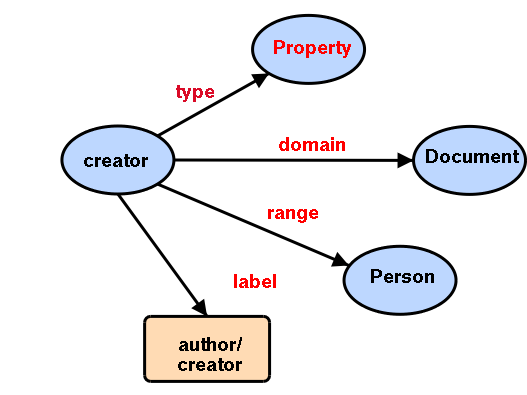
\includegraphics[scale=0.55]{figure2}
%\caption{Popis schémy.}\label{figure2}
%\end{center}\end{figure}
%
%Etiam nec lorem leo, id consequat tellus. Etiam id mattis massa. Phasellus commodo, lacus in viverra lacinia, quam leo ultricies tellus, condimentum vehicula dui nisl a magna. In mi felis, malesuada eget tincidunt eget, rutrum ac lacus. In a nisl tellus. Mauris hendrerit egestas odio ac consequat. Etiam nec lorem leo, id consequat tellus. Etiam id mattis massa. Phasellus commodo, lacus in viverra lacinia, quam leo ultricies tellus, condimentum vehicula dui nisl a magna. In mi felis, malesuada eget tincidunt eget, rutrum ac lacus. In a nisl tellus. Mauris hendrerit egestas odio ac consequat. Etiam nec lorem leo, id consequat tellus. Etiam id mattis massa. Phasellus commodo, lacus in viverra lacinia, quam leo ultricies tellus, condimentum vehicula dui nisl a magna. In mi felis, malesuada eget tincidunt eget, rutrum ac lacus. In a nisl tellus. Mauris hendrerit egestas odio ac consequat.
%
%\lstinputlisting[float=h,language=javascript,caption={Príklad listingu zo súboru.},label={listing},frame=single,frameround=ffff,captionpos=b,basicstyle=\scriptsize]{figures/listing}
%
%Etiam nec lorem leo, id consequat tellus. Etiam id mattis massa. Phasellus commodo, lacus in viverra lacinia, quam leo ultricies tellus, condimentum vehicula dui nisl a magna. In mi felis, malesuada eget tincidunt eget, rutrum ac lacus. In a nisl tellus. Mauris hendrerit egestas odio ac consequat. Etiam nec lorem leo, id consequat tellus. Etiam id mattis massa. Phasellus commodo, lacus in viverra lacinia, quam leo ultricies tellus, condimentum vehicula dui nisl a magna. In mi felis, malesuada eget tincidunt eget, rutrum ac lacus. In a nisl tellus. Mauris hendrerit egestas odio ac consequat. Etiam nec lorem leo, id consequat tellus. Etiam id mattis massa. Phasellus commodo, lacus in viverra lacinia, quam leo ultricies tellus, condimentum vehicula dui nisl a magna. In mi felis, malesuada eget tincidunt eget, rutrum ac lacus. In a nisl tellus. Mauris hendrerit egestas odio ac consequat.
